\section{Formalizing the Bipartisan Paxos Protocols}\seclabel{FormalBPaxosOverview}
In this section, we formalize the BPaxos protocols by way of generalized
consensus on conflict graphs. We begin with a review of conflict graphs and
generalized consensus and then formalize BPaxos graphs and the BPaxos
protocols.

\subsection{Conflict Graphs and Mazurkiewicz Traces}\seclabel{ConflictGraphs}
Consider a set $\Cmd$ of commands and a binary reflexive relation $\conflict$
over $\Cmd$. We say two commands $x, y \in \Cmd$ \defword{conflict} if $(x, y)
\in \conflict$, and we say they are \defword{independent} otherwise. A
\defword{conflict graph}~\cite{mazurkiewicz1995introduction} (with respect to
$\Cmd$ and $\conflict$) is a directed acyclic graph $C = (V, E, \varphi)$ where
\begin{itemize}
  \item
    $V$ is a set of vertices;
  \item
    $E \subseteq V \times V$ is a set of edges;
  \item
    $\varphi: V \to \Cmd$ is a function that labels every vertex with a command;
    and
  \item
    for every pair of vertices $v_1, v_2 \in V$, there exists an edge between
    $v_1$ and $v_2$ if and only if $\varphi(v_1)$ and $\varphi(v_2)$ conflict.
\end{itemize}

We say $C' = (V', E', \varphi|_{V'})$ is a \defword{suffix} of $C$ if $C'$ is a
subgraph of $C$ such that for every edge $(v_1, v_2) \in E$, if $v_1 \in V'$,
then $(v_1, v_2) \in E'$.
%
An example conflict graph is shown in \figref{ExampleConflictGraph} with $\Cmd
= \set{x, y, z}$ and $\conflict = \set{(x, x), (x, y), (y, x), (x, z), (z,
x)}$. Two suffixes of this conflict graph are shown in \figref{ExampleSuffix}
and \figref{ExampleSuffix2}.

\begin{floatingfigure}{0.27\textwidth}
  \centering
  \tikzstyle{vertex}=[]
  \tikzstyle{arrow}=[thick, -latex]
  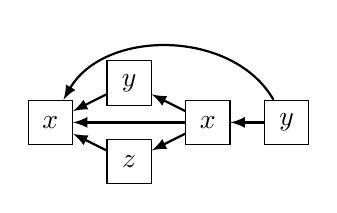
\begin{tikzpicture}
    \node[vertex] (x1) at (0, 0) {$x$};
    \node[vertex] (y1) at (1, 0.5) {$y$};
    \node[vertex] (y2) at (1, -0.5) {$z$};
    \node[vertex] (x2) at (2, 0) {$x$};
    \node[vertex] (z) at (3, 0) {$y$};

    \draw[arrow] (y1) to (x1);
    \draw[arrow] (y2) to (x1);
    \draw[arrow] (x2) to (y1);
    \draw[arrow] (x2) to (y2);
    \draw[arrow] (x2) to (x1);
    \draw[arrow, bend right=60] (z) to (x1);
    \draw[arrow] (z) to (x2);
  \end{tikzpicture}
  \caption{A conflict graph.}\figlabel{ExampleConflictGraph}
\end{floatingfigure}


We associate every conflict graph with the set of command strings that can be
obtained by a reverse topological sort of the conflict graph. For example, the
conflict graph in \figref{ExampleConflictGraph} can be reverse topological
sorted in two ways, yielding the two command strings $xyzxy$ and $xzyxy$.
Notice that these two command strings can be obtained from one another by
interchanging their second and third commands, two commands that do not
conflict. This is true in general. Any two command strings associated with a
conflict graph can be obtained from the other by repeatedly interchanging
adjacent independent commands. These sets of command strings are known as
Mazurkiewicz traces~\cite{mazurkiewicz1985semantics,
mazurkiewicz1995introduction} and formalize the orders in which replicated
state machines can execute commands while remaining in sync.

\subsection{Generalized Consensus}\seclabel{GeneralizedConsensus}
Generalized consensus~\cite{lamport1998part, sutra2011fast} involves a set of
processes known as \defword{learners} attempting to reach consensus on a
growing value. Though generalized consensus is defined in terms of an abstract
data structure known as a command-structure set, we restrict our attention to
generalized consensus on conflict graphs (see \secref{ConflictGraphs}). More
formally, given a set $\Cmd$ of commands and conflict relation $\conflict$, we
consider a set $l_1, l_2, \ldots, l_n$ of learners where each learner $l_i$
manages a conflict graph $C_i$. Over time, a set of client processes propose
commands, and learners add the proposed commands to their conflict graphs such
that the following four conditions are maintained.
\begin{itemize}
  \item \defword{Nontriviality:}
    The vertices of every conflict graph are labelled only with proposed
    commands.
  \item \defword{Stability:}
    Every conflict graph $C_i$ at time $t$ is a suffix of $C_i$ at any time after
    $t$.
  \item \defword{Consistency:}
    For every pair of conflict graphs $C_i$ and $C_j$, there exists a conflict
    graph $C$ such that $C_i$ and $C_j$ are both suffixes of $C$.
  \item \defword{Liveness:}
    If a command is proposed, then eventually every conflict graph contains it.
\end{itemize}



\subsection{BPaxos Graphs and Partial BPaxos Graphs}
Consider a set $\Cmd$ of commands and a symmetric conflict relation
$\conflict$. A \defword{BPaxos graph} (with respect to $\Cmd$ and $\conflict$)
is a directed (potentially cyclic) graph $B = (V, E, \varphi)$ where
\begin{itemize}
  \item
    $V$ is a set of vertices;
  \item
    $E \subseteq V \times V$ is a set of edges;
  \item
    $\varphi: V \to \Cmd$ is a function that labels every vertex with a
    command; and
  \item
    for every pair of vertices $v_1, v_2 \in V$, there exists an edge between
    $v_1$ and $v_2$ if (but not only if) $\varphi(v_1)$ and $\varphi(v_2)$
    conflict.
\end{itemize}
Intuitively, a BPaxos graph is a potentially cyclic conflict graph that can
have spurious edges between vertices labelled with non-conflicting commands.

A \defword{partial BPaxos graph} $B = (V, E, \varphi)$ is a BPaxos graph except
that $\varphi: V \partialto \Cmd$ is partial. Intuitively, a partial BPaxos
graph is a BPaxos graph for which the labels of some vertices are unknown.
%
We say a vertex $v$ in a partial BPaxos graph is \defword{eligible} if $v$ and
all vertices reachable from $v$ are labelled. The \defword{eligible suffix} of
a partial BPaxos graph $B$ is the suffix of $B$ consisting of all eligible
vertices.
%
An example partial BPaxos graph is illustrated in \figref{PartialBPaxosGraph},
and its eligible suffix is shown in \figref{EligibleSuffix}. In this example,
$\Cmd = \set{u, v, w, x, y}$ and
  $\conflict = \set{
    (v, u), (u, v),
    (v, w), (w, v),
    (x, v), (v, x),
    (x, w), (w, x),
    (y, w), (w, y),
    (z, x), (x, z),
    (z, y), (y, z)
  }$.
Note that $B$ in \figref{PartialBPaxosGraph} has an edge between commands $x$
and $y$ even though $x$ and $y$ do not conflict. This is a spurious edge and is
allowed in a partial BPaxos graph but not in a conflict graph. Also note that
command $z$ has an edge to a vertex that is unlabelled.

\begin{figure}[ht]
  \centering
  \tikzstyle{vertex}=[draw, minimum width=16pt, minimum height=16pt]
  \tikzstyle{arrow}=[thick, -latex]

  \begin{subfigure}[b]{2in}
    \centering
    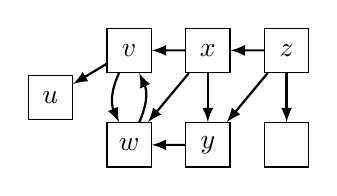
\begin{tikzpicture}[xscale=1, yscale=0.6]
      \node[vertex] (u) at (0, 0) {$u$};
      \node[vertex] (v) at (1, 1) {$v$};
      \node[vertex] (w) at (1, -1) {$w$};
      \node[vertex] (x) at (2, 1) {$x$};
      \node[vertex] (y) at (2, -1) {$y$};
      \node[vertex] (z) at (3, 1) {$z$};
      \node[vertex] (unknown) at (3, -1) {\phantom{z}};

      \draw[arrow] (v) to (u);
      \draw[arrow, bend right=15] (v) to (w);
      \draw[arrow, bend right=15] (w) to (v);
      \draw[arrow] (x) to (v);
      \draw[arrow] (x) to (w);
      \draw[arrow] (x) to (y);
      \draw[arrow] (y) to (w);
      \draw[arrow] (z) to (x);
      \draw[arrow] (z) to (y);
      \draw[arrow] (z) to (unknown);
    \end{tikzpicture}
    \caption{A partial BPaxos graph $B$}\figlabel{PartialBPaxosGraph}
  \end{subfigure}%
  \begin{subfigure}[b]{2in}
    \centering
    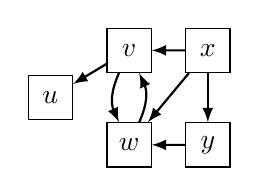
\begin{tikzpicture}[xscale=1, yscale=0.6]
      \node[vertex] (u) at (0, 0) {$u$};
      \node[vertex] (v) at (1, 1) {$v$};
      \node[vertex] (w) at (1, -1) {$w$};
      \node[vertex] (x) at (2, 1) {$x$};
      \node[vertex] (y) at (2, -1) {$y$};

      \draw[arrow] (v) to (u);
      \draw[arrow, bend right=15] (v) to (w);
      \draw[arrow, bend right=15] (w) to (v);
      \draw[arrow] (x) to (v);
      \draw[arrow] (x) to (w);
      \draw[arrow] (x) to (y);
      \draw[arrow] (y) to (w);
    \end{tikzpicture}
    \caption{The eligibile suffix $B'$ of $B$}\figlabel{EligibleSuffix}
  \end{subfigure}%
  \begin{subfigure}[b]{2in}
    \centering
    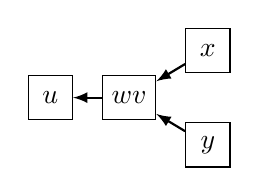
\begin{tikzpicture}[xscale=1, yscale=0.6]
      \node[vertex] (u) at (0, 0) {$u$};
      \node[vertex] (vw) at (1, 0) {$wv$};
      \node[vertex] (x) at (2, 1) {$x$};
      \node[vertex] (y) at (2, -1) {$y$};

      \draw[arrow] (vw) to (u);
      \draw[arrow] (x) to (vw);
      \draw[arrow] (y) to (vw);
    \end{tikzpicture}
    \caption{The condensation of $B'$}\figlabel{Condensation}
  \end{subfigure}

  \caption{}
\end{figure}


The \defword{condensation} of BPaxos graph $B$ is the graph obtained by first
removing spurious edges between non-conflicting vertices in $B$ and then by
contracting every strongly connected component. Every strongly connected
component labelled with commands $x_1, \ldots, x_n$ is replaced with a single
vertex labelled with a command string $x_{i_1} x_{i_2} \cdots x_{i_n}$ that is
obtained from an arbitrary but fixed ordering of the commands $x_1, \ldots,
x_n$.
%
The condensation of a BPaxos graph with respect to $\Cmd$ and $\conflict$ is
a conflict graph with respect to $\Cmd^+$ and $\conflict^+$ where $\Cmd^+$ is
the set of non-empty command strings and where $(x_1 x_2 \cdots x_n, y_1 y_2
\cdots y_m) \in \conflict^+$ if there is some $x_i$ and $y_j$ that conflict in
$\conflict$.
%
An example condensation is shown in \figref{Condensation}. Note that the
spurious edge between $x$ and $y$ was pruned; that the strongly connected
component consisting of commands $v$ and $w$ was contracted into a single
vertex labelled with the command string $wv$; and that the condensation is a
conflict graph.

\subsection{Problem Description}
The BPaxos protocols implement state machine replication by way of generalized
consensus. We assume an asynchronous network model, and we assume that
processes are deterministic and can fail by crashing but cannot act
maliciously. Throughout the paper, we assume at most $f$ processes can fail. We
consider a set $b_1, b_2, \ldots, b_{f+1}$ of deterministic state machine
replicas that all begin in the same initial state. We consider a set $\Cmd$ of
state machine commands and define a conflict relation $\conflict$ such that two
commands $x, y \in \Cmd$ conflict if they do not commute--i.e.\ if there exists
a state in which executing $x$ and then $y$ does not produce the same responses
and final state as executing $y$ and then $x$.

Every BPaxos protocol is a generalized consensus protocol, with state machine
replicas playing the role of learners. Each replica $b_i$ learns a conflict
graph $C_i$ with respect to $\Cmd^+$ and $\conflict^+$. Every replica $b_i$
executes the commands in $C_i$ in reverse topological order as they are
learned. For example, if a replica has learned the conflict graph shown in
\figref{Condensation}, it can execute commands in the order $uwvxy$ or $uwvyx$.
Executing commands in this way, replicas are guaranteed to stay in sync,
producing identical responses for every command they execute.

\subsection{The BPaxos Protocols}
Every BPaxos protocol implements generalized consensus by first reaching
consensus on a partial BPaxos graph.
%
When a client process sends a state machine command $x$ to a BPaxos protocol, a
process implementing the protocol eventually assigns the command to an instance
$I$ and a set of dependencies $\deps{I}$.
%
Instances are called instances because the BPaxos protocol implements one
instance of consensus for every instance $I$. The BPaxos protocol eventually
reaches consensus on the value $(x, \deps{I})$ in instance $I$.  Every state
machine replica $b_i$ maintains a partial BPaxos graph $B_i$ where instances
play the role of vertices. When replica $b_i$ learns that an instance $I$ has
been chosen with value $(x, \deps{I})$, it adds vertex $I$ to $B_i$ labelled
with $x$ and with outbound edges to every instance in $\deps{I}$ (adding
previously unseen instances to $B_i$ as necessary). Letting $C_i$ be the
condensation of the eligible suffix of $B_i$, the BPaxos protocol successfully
implements generalized consensus with replica $b_i$ learning conflict graph
$C_i$ so long as \invref{ConsensusInvariant} and \invref{ConflictInvariant} are
maintained.

\invref{ConsensusInvariant} allows replicas to reach consensus on their partial
BPaxos graphs. \invref{ConflictInvariant} ensures that every replica's partial
BPaxos graph really is a partial BPaxos graph. These two invariants suffice to
ensure stability and consistency for the following reasons.
%
Stability is guaranteed because a replica $b_i$'s partial BPaxos graph $B_i$
(and hence its condensation $C_i$) only grows over time.
%
Consistency is guaranteed because every condensation $C_i$ is a prefix of the
condensation of the eligible suffix of the global partial BPaxos graph, the
graph formed from complete knowledge of every chosen instance.
%
Moreover, the BPaxos protocols do provide liveness with certain assumptions
about the niceness of the network, but we do not focus on liveness in this
paper.
%
Finally, every BPaxos protocol ensures nontriviality in a straightforward way.
